% Template for PLoS
% Version 1.0 January 2009
%
% To compile to pdf, run:
% latex plos.template
% bibtex plos.template
% latex plos.template
% latex plos.template
% dvipdf plos.template

% \documentclass[10pt, twocolumn]{article}
\documentclass[10pt]{article}
\usepackage{amsmath}
\usepackage{amssymb}
\usepackage{graphicx}
\usepackage{color} % for revision purposes only, may be not present in the final file
% cite package, to clean up citations in the main text. Do not remove.
\usepackage{cite}
\usepackage{color}
\usepackage{indentfirst} %% LM: in order to indent the first paragraph of each section
\usepackage{url} %% LM: in order to include nice urls
\usepackage{booktabs} %% LM: nice tables...
\usepackage{subfigure} % LM: panels
\usepackage{xr} % automatic cross-referencing
\externaldocument{Text_S2}
% Use doublespacing - comment out for single spacing
%\usepackage{setspace}
%\doublespacing

\topmargin 0.0cm
\oddsidemargin 0.5cm
\evensidemargin 0.5cm
\textwidth 16cm
\textheight 21cm

\usepackage[labelfont=bf,labelsep=period,justification=raggedright]{caption}

\bibliographystyle{fix/plos2009}% 

\makeatletter
\renewcommand{\@biblabel}[1]{\quad#1.}
\makeatother

\renewcommand{\thesubfigure}{(\Alph{subfigure})}
% Leave date blank
\date{}

\pagestyle{myheadings}
%% ** EDIT HERE **


%% ** EDIT HERE **
%% PLEASE INCLUDE ALL MACROS BELOW

%% END MACROS SECTION

\begin{document}

% Title must be 150 characters or less
\begin{flushleft}
{\Large
\textbf{Spatio-temporal Dynamics of Foot-and-Mouth Disease Virus in South America}
}
% Insert Author names, affiliations and corresponding author email.
\\
Luiz Max Carvalho$^{1,2,3\ast}$,
Nuno Rodrigues Faria$^{4,5}$,
Andres M.~Perez$^{6}$,
Marc A.~Suchard$^{7,8}$
Philippe Lemey$^{4}$,
Waldemir de Castro Silveira$^{2}$,
Andrew Rambaut$^{1,9,10}$,
Guy Baele$^{4}$
\\
\bf{1} Institute of Evolutionary Biology, University of Edinburgh, Edinburgh, United Kingdom.\\
\bf{2} Pan American Center for Foot-and-Mouth Disease (PAHO/WHO), Duque de Caxias, Rio de Janeiro, Brazil.\\
\bf{3} Scientific Computing Program, Oswaldo Cruz Foundation, Rio de Janeiro, Brazil.\\
\bf{4} Department of Microbiology and Immunology, Rega Institute -- KU Leuven, Leuven, Belgium.\\
\bf{5} Department of Zoology, University of Oxford, Oxford, United Kingdom.\\
\bf{6} Department of Veterinary Population Medicine, University of Minnesota, St. Paul, United States of America.\\
\bf{7} Departments of Biomathematics and Human Genetics, David Geffen School of Medicine at UCLA, University of California, Los Angeles,  United States of America.\\
\bf{8} Department of Biostatistics, UCLA Fielding School of Public Health, University of California, Los Angeles,  United States of America.\\
\bf{9}  Fogarty International Center, National Institutes of Health, Bethesda, MD,  United States of America.\\
\bf{10} Centre for Immunology, Infection and Evolution at the University of Edinburgh, Edinburgh, United Kingdom.
$\ast$ E-mail: lm.carvalho@ed.ac.uk
\end{flushleft}
% Please keep the abstract between 250 and 300 words
\section*{Abstract}
Although foot-and-mouth disease virus (FMDV) incidence has decreased in South America over the last years, the pathogen still circulates in the region and the risk of re-emergence in previously FMDV-free areas is a public health concern.
Here we merge environmental, epidemiological and genetic data to reconstruct spatiotemporal patterns and determinants of FMDV serotypes A and O dispersal in South America.
Our dating analysis suggests that serotype A emerged in South America by $\approx1930$, while serotype O $\approx1990$.
The rate of evolution was significantly higher for serotype A compared to serotype O.
Phylogeographic inference identified two well-connected sub networks of viral flow, one including Venezuela, Colombia and Ecuador; another including Brazil, Uruguay and Argentina.
The spread of serotype A was best described by geographic distances, while trade of live cattle was the strongest predictor of serotype O spread.
Our findings show that the two serotypes have different underlying evolutionary and spatial dynamics and may pose different threats to control programmes.

Key-words: Phylogeography, foot-and-mouth disease virus, South America, animal trade.

% \section*{Author Summary} % 150--200 words
% Foot-and-mouth diseases virus (FMDV) is a rapidly evolving and highly infectious livestock pathogen.
% In South America, although some molecular epidemiology studies are available, little is known about the virus phylodynamics.
% In this paper we analyze all available VP1 sequences of FMDV serotypes A and O isolated in South America to unravel the spatial and temporal dynamics of the virus on the continent.
% We show that both serotypes exhibit temporal structure and go on to estimate a time of origin of $\approx 80$ and $\approx 25$ years for serotypes A and O, respectively, and that serotype O presents a dispersal rate four times faster than serotype A.
% Additionally, we find that Venezuela and Brazil are hubs for serotype A spread but not for serotype O, while Colombia and Ecuador seem to be more important for serotype O dispersal on the continent.
% We identify the trade of live cattle as the most important predictor of serotype O, while for serotype A geographic distances seem to best predict viral flow between South American countries.
% Taken together, these results show that the FMDV serotypes' different biology is reflected in their different spatial dispersal patterns and reinforces the view that the trade of live cattle as well as short range migration are important threats to control programs.   

\section*{Introduction}

Foot-and-mouth disease virus (FMDV) is a rapidly evolving picornavirus and the causative agent of foot-and-mouth disease (FMD), the most important disease of domestic and wild cloven-hoofed animals~\cite{review}.
The virus can be classified in seven serotypes, three of which (A, O, and C) have circulated in South America.
Serotype A caused large epidemics throughout the Southern cone in recent years~\cite{Perez2001, Malirat2012}, while endemic circulation has been mostly limited to Venezuela~\cite{Malirat2012}.
Historically, serotype O has been the most prevalent serotype on the continent, but is now limited to areas in the Andean region, and in particular to Ecuador~\cite{andean}.
Serotype C on the other hand was last encountered in the continent in $1995$ in Brazil~\cite{review_eradication}.
Historical reports suggest that FMDV arrived in South America in the late years of the 19th century with European colonization~\cite{Naranjo2013, tully}. 
By the 1970s, FMD was widespread in the region, with several large-scale epidemics being caused by multiple subtypes~\cite{Saraiva2003}.
In South America, FMD control and eradication has traditionally been pursued using a combination of mass vaccination programs~\cite{vaccinationSA} and control of animal movements from areas in which FMDV infection was suspected.
Over time, passive and active surveillance programs have, with different degrees of success, succeeded in the early detection of FMDV.
In order to achieve complete eradication however, the strains involved in epidemics - especially those in previously FMDV-free areas - need to be accurately characterised.

Phylogenetic analyses have proven useful in recovering the transmission pathways from genetic data~\cite{cottam2007, cottam2008} and providing insight into the processes that drive re-emergence~\cite{combining}.
More recently, molecular epidemiology tools have been used to infer the origin and evolutionary history of emerging strains in South America~\cite{Perez2001, Malirat2007, andean, Malirat2011, Maradei2013}.
However, as pointed out by Di Nardo, Knowles \& Paton~\cite{combining}, a common feature of FMDV molecular epidemiology studies is that  joint evaluation of epidemiological, environmental and genetic data has usually been performed outside of an unified quantitative framework.
In face of many sources of information, ranging from genetic data to environmental data on host distribution and outbreak counts, it is desirable to have a framework capable of integrating these sources of information coherently.
Phylodynamics combines population genetics and epidemiology to explicitly  model the interaction between ecological processes such as migration and selection and the shape of the phylogenies~\cite{grenfell, vphylodynamics}.
Bayesian phylodynamics offers an attractive statistical framework to combine multiple sources of information while marginalizing over the topology space, thus accommodating phylogenetic uncertainty.
In particular, phylogeographic methods can be employed to understand viral spatial dynamics under explicit spatial diffusion models~\cite{roots}.
Further, an important research goal is to gain insight into the major determinants of FMDV spread in the continent.
Since animal movements constitute a major threat to eradication programs~\cite{movements}, using animal trade data as predictors can be a valuable tool to understand the role of livestock commerce in the spread of FMDV.
For example, Nelson et al. ~\cite{Nelson2011} coupled swine trade data and genetic data to show swine movements in the United States drove the spread of a novel influenza virus of the H1 subtype.

Here, we investigate the phylodynamic patterns of serotypes A and O in South America using all publicly available VP1 (1D) sequences for those serotypes in South America, sampled over a long time-period (1955-2010 for serotype A and 1994-2010 for serotype O) in nearly all south American countries affected by FMD.
We apply Bayesian phylogeographic methods to investigate the evolutionary dynamics of serotypes A and O in South America incorporating  genetic, spatial and epidemiological data such as livestock trade, geographic distances and vaccination coverage.
This flexible Bayesian phylogeographic framework allows testing hypotheses on viral dispersal, while naturally accommodating phylogenetic uncertainty~\cite{roots, towards}.
We use BEAST~\cite{beast2012} to infer time-structured phylogenies and reconstruct past population dynamics, to which we overlay vaccination and serotype-specific notification data.
To study the factors driving re-emergence, we use data on livestock trade and geographical distances as predictors for viral spatial diffusion and compare competing spatial dynamics models involving each predictor using recently developed methods. 

\section*{Results}

\subsection*{Evolutionary rates and times of origin of FMDV serotypes A and O circulating strains}

First, we performed selection using path-sampling (PS) and stepping-stone (SS) to estimate marginal likelihood and calculate (log) Bayes factors (BF) in order to select the best fitting demographic (tree) model and molecular clock model.
Our results favor a non-parametric skyride model, that allows fluctuations in demographic growth through time, over the constant population size assumption (serotype A: log BF = $11$; serotype O: log BF = $21$).
Using a similar approach, we  found decisive support for the relaxed clock over the strict molecular clock model.
Particularly, the exponential relaxed molecular clock provided a better fit for serotype O data (log BF = $56$) while the log-normal relaxed molecular clock model provided a better fit to serotype A (log BF = $34$) (see Table~\ref{stab:treeclockselection} for details). 
The coefficient of variation for the log-normal relaxed molecular clock model for serotype A had a posterior mean of $0.32$ (95\% highest posterior density [HPD] interval: $0.21$--$0.43$) indicating substantial rate heterogeneity among lineages in the phylogeny.
Root-to-tip plots against sampling times from maximum likelihood phylogenies constructed with PhyML~\cite{phyml} suggested a linear trend (Figure~\ref{sfig:root-to-tip}), which encouraged the pursuit of more detailed estimates.
In addition, we compared a model with and without dated-tips (the `temporal signal' test~\cite{Faria2012, Baele2012}, see Methods) and found significant temporal structure for both serotypes (A: log BF = $310$; O: log BF = $348$), showing that sufficient temporal information is embedded in sequence data of both serotypes under investigation, which is essential for the estimation of divergence times and to reconstruct the population dynamics in natural time units~\cite{MEP}. 

Figure~\ref{fig:trees} shows the maximum clade credibility (MCC) trees estimated for serotype A and serotype O.
The estimated time to most recent common ancestor (tMRCA) of the circulating serotype A strains was $1932$ ($95\%$ HPD: $1925$--$1939$) and  $1989$ ($95\%$ HPD: $ 1986$--$1991$) for serotype O, indicating a more recent origin of the latter. 
Using the combination of best fitting demographic and molecular clock models for each serotype, the evolutionary rate for serotype A was estimated at $\approx 4 \times 10^{-3}$ substitutions/site/year.
The estimated evolutionary rate for serotype O was approximately 2.5 times faster than serotype A, i.e.~at $\approx 1 \times 10^{-2}$, consistent with previous studies~\cite{tully, Carvalho2013, Muellner2011}.
See Text S2, Tables~\ref{stab:SB_A} and~\ref{stab:SB_O} for more detailed estimates.

Figure~\ref{fig:trees}A shows that sequences from the same country tend to cluster in small clades, although the inferred phylogenies for both serotypes also show considerable interspersing of lineages, indicating trans-border FMDV spread.
For example, Argentinian serotype A sequences were grouped in two clades, that either comprised only Argentinian isolates or included sequences from Brazil and Uruguay (Figure~\ref{fig:trees}A).
Interestingly, the majority of the isolates from Venezuela and Colombia fall together within two distinct clades.
For serotype O there is also interspersing of clades from different locations, with one large clade featuring interleaved Ecuadorian and Colombian clades (Figure~\ref{fig:trees}B).
A smaller clade of Colombian isolates are found interspersed within Venezuelan isolates.
In addition, isolates from Ecuador were grouped with isolates from Colombia, suggesting that the intra-country dynamics of FMDV between these two countries is intrinsically linked.
These observations indicate that there is spatial structure in the data, i.e., that there is association between phylogeny and geography.
We further explore this using the Bayesian Tip-Significance testing (BaTS)~\cite{bats} to calculate phylogeny-trait association indexes such as the parsimony score (PS), association index (AI) and maximum clade size (MC) (see Text S2 for details).
Both serotypes show significant (randomised p-value $< 0.05$) location-tip association for the three indexes (Table~\ref{stab:BaTS}).
As an overall summary, our data sets present a high degree of spatial signal, justifying richer phylogeographic analyses to study the transmission network of FMDV on the continent.

\begin{center}
 [Figure~\ref{fig:trees} about here]
\end{center}

\subsection*{Spatial Dynamics of FMDV in South America}

To gain insight into the spatio-temporal process of FMDV spread, we employed an asymmetric continuous-time Markov chain (CTMC) phylogeographic model~\cite{roots} implemented in BEAST~\cite{beast2012}, coupled with model averaging using a Bayesian stochastic search variable selection (BSSVS) procedure.
Spatial projections of the maximum clade credibility trees (Figure~\ref{fig:migration}) show that Brazil and Colombia were the most strongly connected regions (hubs) both for serotypes A and O, respectively. 
In the serotype A phylogeography, Brazil is connected to Argentina, Uruguay, Venezuela and Colombia, while for serotype O, Colombia was connected to Venezuela, Ecuador and Bolivia.
These results suggest different spatial patterns for the two serotypes.

We observe that for serotype A mainly long-range migration routes were inferred for the period before $1945$.
This may however result from the limited amount of data available before $1970$, which limits accurate inference migration events back in the past (see \textbf{Discussion}).
Also, there is a major expansion in spatial spread from $1945$ to $1965$, characterized by Brazil as a source of virus for the rest of the continent.
In the period $1965-1980$, we observe a slower spread, mainly through short range routes.
The $1980-2008$ window is characterised by FMDV serotype A flow into Peru and Paraguay and the increase of intra-country diversity (depicted by the radius of the displayed circles in Figure~\ref{fig:migration}).   

On the other hand, the serotype O expansion seems to have occurred in the mid $1990$'s.
Up to 1995, our reconstruction suggests that Colombia and Brazil appear to act as primary and secondary viral sources, respectively.
From 1995 to $2000$, whilst Colombia acted as the main source for the northern/Andean regions of the continent, the spread to the Southern Cone seems to stem from Brazil.
The period $2000-2010$ is characterized by a decrease in viral dispersal movements (almost no new edges added to the network) concomitant with an increase in viral diversity within countries, specially Ecuador, Colombia and Brazil.

We then looked at the statistical support for epidemiological linkage between pairs of locations using Bayes factors~\cite{roots}.
For serotype A we found high statistical support for viral migration between Uruguay and Argentina (BF = $985$), Venezuela and Colombia (BF = $812$), Bolivia and Brazil (BF = $25$) and Brazil and Argentina (BF = $6$).
On the other hand, for serotype O the most supported links were between Colombia and Ecuador (BF = $557$), Ecuador and Peru (BF = $223$),  Venezuela and Colombia (BF = $52$), Paraguay and Argentina (BF = $6$). 

\begin{center}
 [Figure~\ref{fig:migration} about here]
\end{center}

To infer which countries have most significantly contributed to the dispersal of FMDV serotypes, we estimated net migration flow (efflux - influx) using a robust counting approach~\cite{Minin2008}.
Figure~\ref{fig:mj&BFs} shows that the supported migration routes differ for each serotype, with some overlapping routes connecting Venezuela and Colombia. 
We also noticed that the pattern of emitters/receivers is different for each serotype.
While for serotype A Brazil and Argentina acted mainly as viral exporters, Venezuela and Bolivia presented the highest net rates for serotype O.
Overall, net migration rates were substantially higher for serotype A in comparison to serotype O (Figure~\ref{fig:mj&BFs}).
The presence of Bolivia as a viral hub for serotype O dispersal and its negligible role for serotype A  dispersal is an interesting difference between the two serotypes. 
Likewise, Brazil is highly connected in the serotype A network but not on the serotype O network.

\subsubsection*{Preferential Spread of FMDV across neighbouring countries}
We compared the transition counts between countries that share borders and those which do not and found that for serotype A the posterior median transition count between neighboring countries was  $22$ (95 \% HPD: $17$--$27$) while ``non-border'' transitions had a posterior median of $4$ (95~\% HPD: $0$--$7$). For serotype O, similar results were observed, with $16$ ($13$--$20$) and $1$ ($0$--$3$) location-transitions being observed for border (B) and non-bordering (NB) countries, respectively.
Considering each South American country as a possible discrete state, there are  possible transitions ($34$ B AND $38$ NB transitions)
For serotype A, the figures have to be adjusted because we have samples from $8$ countries, resulting in $B = 26$ and $ \text{NB} = 30$.
Of course, these estimates have to be compared with their prior expectations
Remarkably, however, the importance of long-range migration routes seems to differ for both serotypes, since the posterior median proportion of ``non-border'' transitions is considerably different (A: $0.14$, $0.00$--$0.28$  and O: $0.05$, $0.00$--$0.20$).

\begin{center}
 [Figure~\ref{fig:mj&BFs} about here]
\end{center}

\subsubsection*{Spatial origins for main South American FMDV outbreaks}

Figure~\ref{fig:epidemictracing} shows the posterior distribution of the location of origin for some epidemics of interest.
The most probable origin of the strains isolated in Argentina $2001$ (Figure~\ref{fig:epidemictracing}A) was Argentina (posterior probability = $0.72$) while Brazil received $0.28$ posterior probability.
Results for the Brazilian strains of the same year point to Argentina as the source of the epidemic with high probability, confirming the strong link between the two countries (Figure~\ref{sfig:epitrac}B).
However, these results should be interpreted with caution due to the low number of sequences from Uruguay.
Contrasting to the connectivity with Argentina, Bolivia $2001$ seems to have had an independent introduction from Peru, as shown in Figure~\ref{sfig:epitrac}C
We provide evidence of Venezuela as a major viral source for serotype A in its region in Figure~\ref{fig:epidemictracing}B, where we show the origins of the Ecuadorian strain isolated in $2002$.
This notion of Venezuela as a seeder is further strengthened by the fact that the Colombian $2008$ strain was most likely imported from Venezuela (posterior probability $\approx 1$, shown in Figure~\ref{sfig:epitrac}D).

Similar to what was found for Venezuela and serotype A, Colombia seems to be the source of most of the strains circulating on the northern part of South America.
As with the introduction of serotype A in Colombia in $2008$, the strains from Venezuela $2003$ have high probability of being imported from Colombia (Figure~\ref{fig:epidemictracing}D).
Consistent with these findings, Figures~\ref{sfig:epitrac}B and~\ref{sfig:epitrac}C we show that Colombia was the most probable origin of the strains in Ecuador ($2002$).
The link between Venezuela and Colombia thus seems to be supported from data for both serotypes, although the main viral seeder varies for each serotype (see \textbf{Discussion}).

\begin{center}
 [Figure~\ref{fig:epidemictracing} about here]
\end{center}

To address the relevance of epidemiological predictors, such as geographic distance and livestock trade on viral diffusion, we collected data on the trade of live cattle, pigs and sheep  as well as geographic distances, and then estimated marginal likelihoods for each of these predictors.
The sub-network connecting Venezuela, Colombia and Ecuador is present in all three graphs.
Similarly, Southern Cone countries are also connected in the three networks.
Additionally, for the sheep and cattle networks, we identified some long-range trade routes, for instance the trade of sheep between Argentina and Colombia.
We used geographic distances as well as the data on the trade of livestock to specify CMTC rate matrix priors (potential predictors), and we use PS/SS to calculate (log) marginal likelihoods for each predictor to determine the importance of each variable for viral spread~\cite{Carvalho2013, Nelson2011}.
While for serotype A the best predictor was the geographic distance between countries (log BF$\approx 4$, compared to the equal-rates gamma prior), the exchange of cattle was the best predictor for serotype O spread (log BF$\approx 13$). 
Also, while for serotype A we found moderate statistical support for geographic distances as predictors of viral spread, this predictor had higher statistical support for serotype O (log BF$\approx 9$).

\begin{center}
 [Table~\ref{tab:preds} about here]
\end{center}

For each predictor, we also assessed the location state distribution at root. 
This vector gives the posterior probability of each country being the origin of the circulating strains.
In Table~\ref{tab:roots} we show that for serotype A there was discordance between predictors about which country was the most probable source of FMDV on the continent.
Peru was the most probable location of origin for the `cattle' predictor, but notably not for the best fitting predictor (geographic distance), for which Argentina was estimated as the origin with moderate probability ($0.75$).
Argentina was also the most probable root for the equal-rates gamma prior model ($Pr(\text{root})=0.84$).
For the swine trade predictors, Colombia was found to be the spatial origin.
For serotype O, predictors showed much more concordance, and Colombia was pointed out as the spatial viral origin for all predictors with high probability (Table~\ref{tab:roots}).
Regarding spatial signal extraction, as measured by the Kullback-Liebler (KL) divergence (relative  to a uniform prior) at the root~\cite{roots} (see also Text S2) for each predictor, we found KL divergences ranging from $3.86$ to $5.91$, showing highly concentrated distributions at the root. 
The predictors with highest KL divergences  were pigs and sheep for serotypes A and O respectively.
The results for serotype A are therefore inconclusive since the most efficient predictor (pigs) pointed a different origin than the best fitting predictor (distance).
Further studies will be necessary to address the spatial origins of FMDV serotype A in South America.

\begin{center}
 [Table~\ref{tab:roots} about here]
\end{center}
\subsubsection*{Sensitivity analysis of spatial sampling heterogeneity}

Since our data sets contain unbalanced geographic samples (Table~\ref{stab:reps}), we conducted a detailed sensitivity analysis to assess the robustness of our results to over-representation of some locations~\cite{Faria2012, fluPNAS, Bedford2010, polar}.
We randomly draw five sequence sub-samples for each serotype in which over-represented geographic regions were down-sampled and run the asymmetric CTMC (with BSSVS) analysis for each sub-sample.
We calculated log Bayes factors and observed good agreement between sub-samples in terms of supported routes for both serotypes (see Figures~\ref{sfig:bssvsA} and~\ref{sfig:bssvsO}). 

To further investigate the agreement between sub-samples, i.e., if parameter estimates were consistent across subsamples, we also computed the $L_1$ matrix distance norm across the estimated posterior mean rate matrices for each sub-sample, and no aberrant samples were detected (see Text S2 for detailed results).
Another aspect of interest is the amount of information extracted from each sample, which we measure by calculating Kullback-Leibler~\cite{KL} divergence between prior and posterior distributions of spatial location at root~\cite{roots}.
Tables~\ref{stab:ED_A} and~\ref{stab:ED_O} show that for all sub-samples in both serotypes, there was lower information extraction when compared to the full analysis, with moderately concentrated posterior distributions at root.
This result is expected, because each subsample has less data than the full data set.
For serotype O, inference about location of origin was consistent across samples, with Venezuela being the most probable country of origin.
In the case of serotype A, however, there was some disagreement about the most probable root state, with Argentina being pointed as root by one of the sub-samples.
Also, we observe very similar support for Venezuela as root for serotype O when compared to Brazil as root for serotype A.
While serotype O presented average probability that Venezuela was the root of $0.47$, the average probability that Brazil was the root for serotype A was $0.50$.
We take the lack of agreement between the distribution at root for the sub-samples and the results from the full data to be the result of the lack of information in the down-sampled analyses, as evidenced by the much lower KL divergences (Tables~\ref{stab:ED_A} and~\ref{stab:ED_O}). 

\subsection*{Demographic reconstruction of FMDV}

The demographic reconstruction using the non-parametric skyride coalescent model shows strikingly different dynamical behavior for the two serotypes (Figure~\ref{fig:skyride}).
While serotype O exhibits a peak diversity in the late years of the 1990's, the diversity of serotype A has been slowly decreasing over the last $20$ years.
Serotype A exhibits a more stable behavior over most of the 20th century, with most variation occurring within the temporal sampling interval, mainly in the last years of the 2000s.
To gain insight into the relationship between vaccination and viral diversity, we overlaid vaccination data to the skyride plots presented in the yellow line in Figure~\ref{fig:skyride}.
These data were expressed as (log) doses per head, which we consider to be a more accurate measure of vaccination coverage, since it corrects for population size increase/decrease over time (see Figure~\ref{sfig:prod} for livestock population time series). 

Further, serotype-specific disease notification (number of cases) data was overlaid on the demographic reconstruction to illustrate the relationship between viral diversity and the onset of epidemics. 
For serotype A, we observe a bottleneck of viral diversity around $2001$ (red line) that coincides with a major epidemic by this serotype that affected several countries in the period $2000-2002$, especially Argentina.
The effective population size for serotype O (blue line) shows a different, more steady pattern over the years, with diversity reaching its lowest level by end of the years $2000$.
This decreasing trend in viral diversity is also observed for serotype A.
The number of vaccine doses shows a marked increase after $2001$ (note that the Y-axis in Figure~\ref{fig:skyride} in natural log units), and the number of cases also declines for both serotypes, in particular for serotype A.
Although we do not provide any formal association analysis, the general intuition is that increasing vaccination efforts as well as other preventive measures decisively decreased transmission and thus viral diversity.
Finally, to assess the robustness of our reconstructions we performed demographic reconstructions using a) only recent (sampling date $>2000$) sequences (see Text S2, Figure ~\ref{sfig:only2000sky}) and b) data sets without the over-represented locations (data not shown).
These analyses gave very similar results to those presented in Figure~\ref{fig:skyride}.

\begin{center}
 [Figure~\ref{fig:skyride} about here]
\end{center}


\section*{Discussion}

In this paper we study the spatio-temporal evolutionary dynamics of FMDV serotypes A and O in South America, using state-of-the-art Bayesian phylogenetic methods to uncover the similarities and differences between these serotypes and assess the impact of their different biology on their population dynamics.
We identified important differences in evolutionary tempo and mode between serotypes, with different countries being important for spread.
These differences in evolutionary rate magnitude and variability suggest that, although the two serotypes share the same host range and infection routes, they present rather different evolutionary dynamics in the continent, which may help explaining their different emergence patterns (see Figure 3 in Naranjo \& Cosivi, 2013~\cite{Naranjo2013}). 

For serotype A, the spread of the virus into  Brazil, Colombia and Venezuela seems to take place in the early decades of the 20th century while the introduction into Uruguay and Paraguay seems to take place much later, suggesting the former as original viral reservoirs and the latter as viral importers.
The spread of the serotype O strains  circulating in South America begins in Colombia around $1994$ and quickly disperses to neighbouring countries such as Ecuador and Venezuela, suggesting that the strains circulating during the 2000s may have been introduced from elsewhere.
Our analysis however indicates that the strains isolated in Colombia in $1994$ are at the root of the circulating serotype O strains in the continent (Figure~\ref{fig:epidemictracing}).
The inclusion of archival sequences from other continents would make it possible to determine whether the circulating strains are the result of sustained maintenance or the result from multiple introductions. 

We found well-supported migration paths between Venezuela, Colombia and Ecuador for both serotypes indicating an important spread pathway in the northern part of South America, with Argentina, Brazil and Uruguay forming a well-supported (BFs $> 9$) sub-network (see Figure~\ref{fig:mj&BFs}).
Interestingly, for serotype O the Markov jumps analysis shows a clear separation in two sub-networks (Figure~\ref{fig:mj&BFs}), one comprising the Southern cone and the other comprising Andean countries.
This separation suggests that viral transmission may follow different regimes in these two regions, which have different forms of livestock production~\cite{Saraiva2003,Naranjo2013}.
The link between these two sub-networks appears to be Bolivia, where viral introduction took place around $2000$, most likely came from Peru (Figure~\ref{sfig:epitrac}). 
Since both Peru, Bolivia and Venezuela are considered to have achieved less than expected regarding the implementation of control measures~\cite{Naranjo2013}, a link passing through these countries is plausible.
The northern (Andean) part of South America also stands as a major diversity reservoir for FMDV, with Colombia being the main viral seeder for serotype O and Venezuela being decisively important for serotype A maintenance in its region.
It should be stressed however that while Colombia has taken the appropriate steps to controlling FMD in its territory, Venezuela still faces challenges in implementing the necessary control policies~\cite{Naranjo2013}.

Using data on trade of live cattle, pigs and sheep between South American countries as predictors of FMDV diffusion provides further evidence of different factors influencing the spread of serotypes A and O.
The trade of cattle was the most significant predictor for serotype O spread, what is compatible with the notion that these hosts are the most important for FMDV maintenance and transmission, even though sheep population sizes are on par with those of cattle~\cite{Saraiva2003}.
Distance between countries was also an important predictor of spread, a result consistent with the finding the most location-transitions occur between countries that share borders.

Previous studies have shown that occurrences caused by serotype A present longer cycles and wider epidemics, while serotype O is more prevalent with shorter disease cycles~\cite{colombiatime}.
These epidemiological features are reflected in the temporal variation observed for viral $Ne$ in both serotypes, a result obtained for other viruses as well~\cite{Bennett2010,Pybus2003}. 
The diversity bottleneck observed for serotype A in Figure~\ref{fig:skyride} is consistent with a single strain being rapidly transmitted during the epidemic that affected several countries during $2000-2002$.
Combined with the results from the epidemic tracing presented in Figures~\ref{fig:epidemictracing} and~\ref{sfig:epitrac}, which show that Argentina most likely seeded the outbreaks in Brazil and Uruguay, he demographic histories presented here provide additional evidence of transborder diffusion as an important factor driving re-emergence in previously FMDV-free areas, as were Argentina and Uruguay at the time, for example.
The demographic reconstruction for serotype O does not show any bottlenecks, suggesting a different epidemiological scenario, in which viral introductions lead to establishment of endemicity and increased viral diversity.
Our results suggest that this serotype O lineage was introduced in Ecuador from Colombia (Figure~\ref{sfig:epitrac}E) and then underwent endemic circulation.

Overall, both spatial and temporal analyses point towards serotype O circulation in South America being characterized by endemic establishment with smaller epidemics and increased viral persistence. 
We found that Colombia was the most probable location of origin for serotype O, a result consistent with  Carvalho et al. ~\cite{Carvalho2013}, that showed that a province close to the border with Colombia, where an annual animal fair takes place, was the most probable spatial origin of the strains circulating in Ecuador from $2002$ to $2010$.
Serotype A on the other hand shows lower within country diversity and seems to occur in bursts, marked by rapid trans-border spread and larger outbreaks. 
Despite these important differences, from the temporal reconstructions for both serotypes it can be noticed that over time, with the increase of vaccination coverage, viral effective population size ($Ne$) decreases dramatically, a result previously obtained for serotype O in Ecuador~\cite{Carvalho2013}.
Vaccination seems to be disrupting viral diversity, likely by precluding spread over large spatial extents, inducing a state of focalised transmission.
Since our results suggest that these two serotypes present rather different evolutionary dynamics, the overall decrease in viral diversity detected for both serotypes points towards a progressive success of the eradication program in slowly reducing transmission and viral diversity.

\section*{Methods}

\subsection*{Genetic and epidemiological data}

To study the spatio-temporal spread dynamics of FMDV within South America, we compiled the largest database of 1D (VP1) gene sequences to date for serotypes A and O.
We retrieved all 1D (VP1) nucleotide sequences available from the National Center for Biotechnology Information (NCBI, \url{ http://www.ncbi.nlm.nih.gov/}) for which there was information on country and year of isolation.
This resulted in 131 sequences (from eight countries) for serotype A and 167 sequences (from nine countries) for serotype O, covering time spans of 55 (1955-2008) and 16 (1994-2010) years, respectively (see Text S1 for details).
Each data set was aligned using the MUSCLE~\cite{muscle} algorithm implemented in the MEGA5~\cite{MEGA} package.

Data on animal trade were obtained from the FAO database (\url{http://faostat.fao.org/}).
We retrieved data on the detailed trade matrix for cattle, pigs and sheep (number of live animals exchanged) covering the period from 1986 to 2009, for each of the nine countries.
Serotype-specific outbreak notifications were obtained from FMD Bioportal (\url{http://fmdbioportal.ucdavis.edu:8080/}).

\subsection*{Phylogenetic Analysis}

Both data sets were checked for recombination using the SBOP and GARD~\cite{sbpgard} tools available from the Datamonkey facility (\url{http://www.datamonkey.org/}), which did not yield any indications of recombination being present in our data sets.
For all our analyses, a general time reversible (GTR)~\cite{Tavare1986} model of sequence evolution was assumed, along with Gamma distributed rate heterogeneity (4 categories).
We take a Bayesian approach to testing evolutionary hypotheses while accommodating phylogenetic uncertainty. 
To this end, we used the Bayesian Evolutionary Analysis by Sampling Trees (BEAST)~\cite{beast2012} software package to infer time-structured phylogenies for the two serotypes taking advantage of the  BEAGLE~\cite{BEAGLE} library to gain computational efficiency.
To compare the performance of several combinations of tree priors and molecular clocks for each data set (see Text S2), we used state-of-the-art marginal likelihood estimators, such as path sampling (PS)~\cite{LartillotPhilippe} and stepping-stone sampling (SS)~\cite{Xie}, which have only recently been introduced in the field of phylogenetics~\cite{LartillotPhilippe, Xie, Baele2012, Baele2013a, Baele2013b, Baele2013c}.

\subsection*{Quantifying temporal and spatial signal} 

To assess the temporal signal for each serotype, we used the approach described in Faria et al.~\cite{Faria2012} and Baele et. al~\cite{Baele2012} and compared the marginal likelihoods of a dated-tips model and a contemporaneous-tips model by calculating Bayes Factors (BF)~\cite{Suchard2001, suchard2005models} (see Spatial Model Selection for details).
We followed Kass and Raftery (1995)~\cite{KassRaftery1995} and considered a log BF$>$3 to be indicative of decisive support for the hypothesis of temporal structure.

Spatial signal was quantified using Bayesian tip-association tests, implemented through the BaTS software package~\cite{bats}.
To detect phylogeny-location association, each sequence was assigned to its country of origin and we computed association index (AI) and parsimony score (PI) using BaTS on  a subset of 1000 samples from the posterior distribution of topologies.
We obtained a null distribution for each statistic (AI and PI), against which the observed indices were compared and significance was assessed.
Additionally, we computed the monophyletic clade (MC) size for each state (country), as a local indicator of phylogeny-trait association for each state (country).
Please see Text S2 for further details on the BaTs analyses.

\subsection*{Spatio-temporal Dynamics}

We apply the non-parametric skyride coalescent model~\cite{skyride} in order to reconstruct the past population dynamics for both serotypes, using a Gaussian Markov Random Field (GMRF) prior to obtain smooth estimates for effective population size trajectories over time.
To gain insight into the mechanisms driving viral dynamics, we overlay the demographic reconstructions to serotype-specific outbreak and vaccination (doses per head) time series.
Phylogeographic analyses of FMDV in South America were performed using the methods presented in Lemey et al.~\cite{roots}, available in BEAST. 
An asymmetric, non-reversible discrete phylogeographic model was applied to both data sets, with each country used as a discrete state.
For statistical efficiency, we used Bayesian stochastic search variable selection (BSSVS) to choose the minimal set of dispersal rates that sufficiently explain the observed data.
BSSVS naturally allows for assessing the significance of each migration route through a Bayes factor (BF) test.
We used SPREAD~\cite{spread} to generate KML files (visualized using Google Earth, \url{http://www.google.com/earth/index.html}) and calculate BFs for statistically significant epidemiological links between discrete locations.
We then computed the expected number of transitions between each pair of locations conditional on the observed data and summarize the number of transitions between countries using a robust counting approach~\cite{Minin2008}.
For these analyses we used a sample of $10,000$ trees from the posterior distribution of topologies.
Unbalanced sampling can have an important impact on the inference of the spatial migration rates~\cite{Faria2012, Lemey2014, Frost2014}
In this study, both data sets analyzed presented highly preferential sampling, with Ecuadorian sequences representing about 50\% of the serotype O data and about 45\% of serotype A sequences being from Argentina (see Text S1 for details).
We therefore conducted an extensive sensitivity analysis, exploring various sampling schemes and comparing the obtained parameter estimates.
Supplementary Text S2 shows a complete description of the parameter estimates under different sampling schemes. 

\subsubsection*{Spatial Model Selection}

In this study we exploit recent developments in Bayesian model selection~\cite{Baele2012, Baele2013a, Baele2013b, Baele2013c}, as implemented in the BEAST software program~\cite{beast2012} to compare the different epidemiological predictors.
Specifically, we perform accurate estimation of the (log) marginal likelihood using path sampling (PS)~\cite{LartillotPhilippe} and stepping-stone sampling (SS)~\cite{Xie}, two computationally demanding approaches that yield accurate estimates of model fit while accommodating phylogenetic uncertainty.
Using these (log) marginal likelihoods, it is possible to calculate Bayes Factors, which provide a measure of the relative performance of each model. 
All (log) marginal likelihood estimations in this study were performed using 64 power posteriors, which were each run for 2 million iterations, taking up to 4 weeks of (wall time) computation for each model under evaluation. 
Using PS and SS, we first compared different demographic priors and clock models (see Supplementary Text S2) for both serotypes. 
For more details on these model selection procedures please see Supplementary Text S2.

To test the influence of different epidemiological predictors on viral diffusion through space, we used trade of live cattle, pigs and sheep to parameterize priors for the CTMC rate matrix.
The numbers of live animals exchanged between countries were normalized to have mean and coefficient of variation of $1$ and used as prior expectations in BEAST (see~\cite{roots}, pg. 14 and the Appendix in~\cite{Carvalho2013}).  
We compared these predictors to a distance-informed prior~\cite{roots}, which represents a scenario where flow occurs as a function of the inverse of the geographic distances between locations.
Finally, all predictors were compared against an equal-rates gamma prior, which considers~\textit{a priori} a scenario where there is no preferential spread among different countries~\cite{Nelson2011}.

\section*{Acknowledgments}
The authors would like to thank Ant\^onio Mendes (PANAFTOSA) for clarifications regarding the vaccination data, Matthew Hall (Edinburgh) and Oliver Pybus (Oxford) for insightful contributions and Miguel Carvalho, Felipe Figueiredo (PROCC) and Mauricio Oliveira (UFRJ) for operational support.
We acknowledge the support of the National Evolutionary Synthesis Center (NESCent) through a working group (Software for Bayesian Evolutionary Analysis).

\emph{Funding:} The research leading to these results has received funding from the European Union Seventh Framework Programme [FP7/2007-2013] under Grant Agreement no. 278433-PREDEMICS and ERC Grant agreement no. 260864.
This work was also supported by National Institutes of Health grants R01 HG006139 and National Science Foundation grants DMS 1264153.

\emph{Conflict of Interest:} none declared

\newpage
\bibliography{FMDV_AMERICA}
% \newpage
\section*{Figure Legends}


{\bf Figure~\ref{fig:trees}. Phylogenetic relationships of foot-and-mouth disease virus (FMDV) serotypes A and O isolates from South America.} Time-scaled phylogenetic maximum clade credibility (MCC) trees for FMDV VP1 sequences from eight countries in the period 1955-2010 for serotype A (Panel A) and nine countries 1994-2010 for serotype O (Panel B).
Tips were collapsed for clarity and colored according to geographic origin.
Diamonds sizes are proportional to posterior probabilities.
From these it is clear that there is considerable interspersing of sequences from different locations within clades.
In particular, Colombian and Ecuadorian sequences form mixed clades in both phylogenies.
The tree for serotype A (panel A) shows considerably more interspersing than the one for serotype O (panel B), but overall both phylogenies suggest a considerable degree of spatial mixing.

{\bf Figure~\ref{fig:migration}. Spatio-temporal dynamics of FMDV in South America} Using an asymmetric diffusion model, we reconstructed the spatial spread of FMDV serotypes A and O throughout the South American continent during the 20th century.
The figure presents spatial projections of the maximum clade credibility trees produced with SPREAD~\cite{spread} and visualized using Google Earth (\url{http://www.google.com/earth/index.html}).
Circle radius are proportional to lineage diversity.
For serotype A (left hand panels), some long-range migration events took place in the period $1945-1965$ and may have led to the establishment of viral circulation in the Souther cone.
Contrasting to this, for serotype O dispersal from the Nother part of the continent to the Southern Cone seems to have been bridged through Bolivia (panel B).
Regarding diversity, Colombia, Venezuela and Ecuador stand out as the main reservoirs of viral diversity for both serotypes.

{\bf Figure~\ref{fig:mj&BFs}. Migration networks for FMDV serotypes A and O in South America.} We estimated the number of migration events between countries using the robust counting (Markov jumps) techinique of~\cite{Minin2008}.
Additionally, a separate analysis employing Bayesian Stochastic Search Variable Selection (BSSVS) was performed to determine most significant migration routes and Bayes factors are depicted by arrows, with line thickness proportional to BF magnitude.
We only plot BFs bigger than $3$.
Coroplethic maps show the net migration rates for each country, for both serotypes.
From this it is clear that the pattern of spatial spread is different for both serotypes, although there is agreement on the likage between Venezuela and Colombia and Ecuador and Peru.
For serotype O, Bolivia stands out as a hub, while for serotype A Brazil is highly connected.
Also notice that exchange rates (depicted by the colors) are considerably higher for serotype A.

{\bf Figure~\ref{fig:epidemictracing}. Epidemic tracing using robust counting for serotypes A and O in South America.} We show the most probable sources of serotype A epidemics in Argentina 2001 (A) and Ecuador 2002 (B).
For serotype O the origins of  all the Colombian sequences from 1994 (C) are shown along with the origins of the strain in Venezuela 2003 (D).
The strains in the Argentinian $2001$ outbreak were probably already circulating in the country (panel A), while the strains isolated in Ecuador $2002$ were most likely originated in Venezuela (panel B) rather then in Argentina, where a major outbreak had occurred the previous year.
For serotype O, the circulation in Colombia has most likely being occurring since before $1994$ (panel C).
In addition to being the most probable root of the circulating strains, Colombia seems also to have seeded the introduction of serotype O in Venezuela around $2003$ (panel D).

{\bf Figure~\ref{fig:skyride}. Temporal dynamics of FMDV serotypes A and O in South America.} Population dynamics were reconstructed for both serotypes using the Gaussian Markov Random Field (Skyride) prior (see Methods).
Additionally, data on vaccination (doses per head) and (log) FMD serotype-specific notifications were superimposed on the demographic reconstruction, with 95 \% Bayesian credible intervals shaded in gray.
Combined with the results from the epidemic tracing presented in Figures~\ref{fig:epidemictracing} and~\ref{sfig:epitrac}, which show that Argentina most likely seeded the outbreaks in Brazil and Uruguay, this provides additional evidence of transborder diffusion as a factor driving re-emergence in previously FMDV-free areas.
The demographic reconstruction for serotype O does not show any bottlenecks, suggesting a different epidemiological scenario, in which viral introductions lead to establishment of endemicity and increased viral diversity .
Since our results suggest that these two serotypes present rather different evolutionary dynamics, the overall decrease in viral diversity detected for both serotypes points towards a progressive success of the eradication program in slowly reducing transmission and viral diversity.

\newpage
\section{Figures and Tables}
%%%%%%%%%%%%%%%%%%%%%%%%%%
%%%%%%%%%%%%%%%%%%%%%%%%%%
\begin{figure}[!ht]
\begin{center}
\subfigure[A]{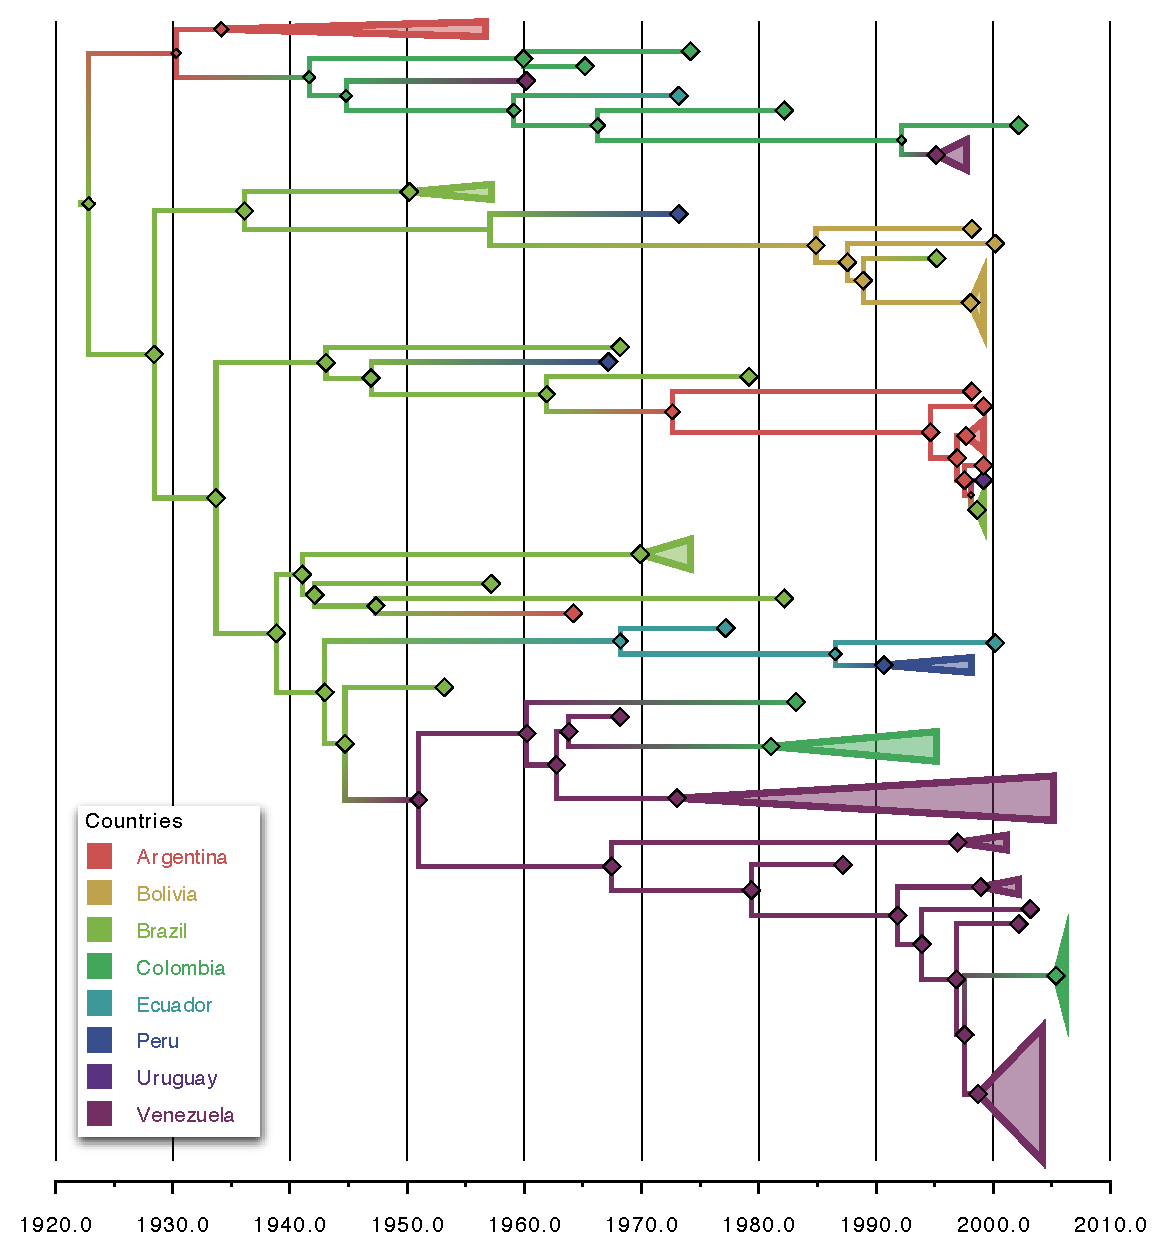
\includegraphics[scale=.45]{FIGURES/A.pdf}}\\
\subfigure[O]{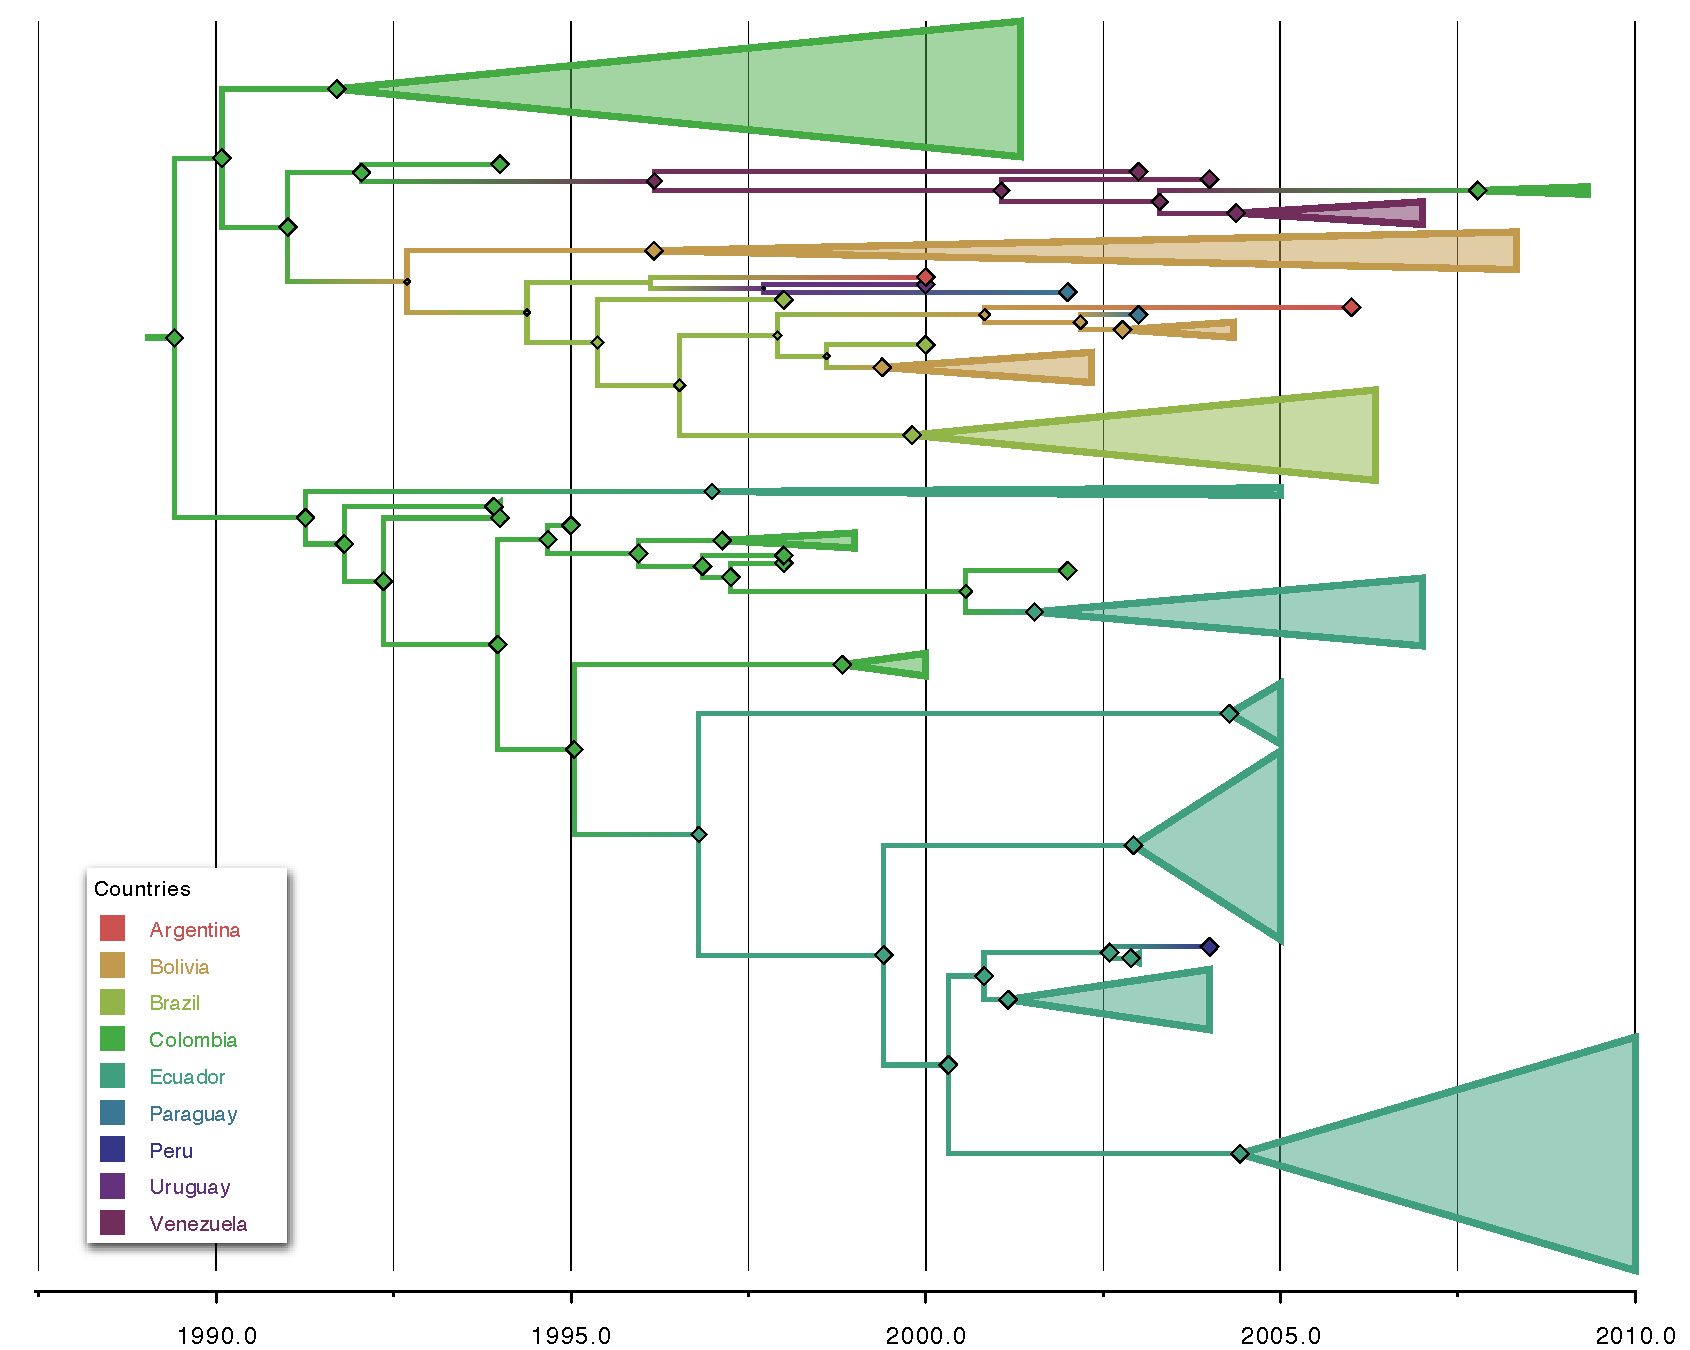
\includegraphics[scale=.30]{FIGURES/O.pdf}}
\end{center}
\caption{}
\label{fig:trees}
\end{figure}
%%%%%%%%%%%%%%%%%%%%%%%%%%
%%%%%%%%%%%%%%%%%%%%%%%%%%
\newpage
\begin{figure}[H]
\begin{center}
\subfigure[A -- $1945$ ]{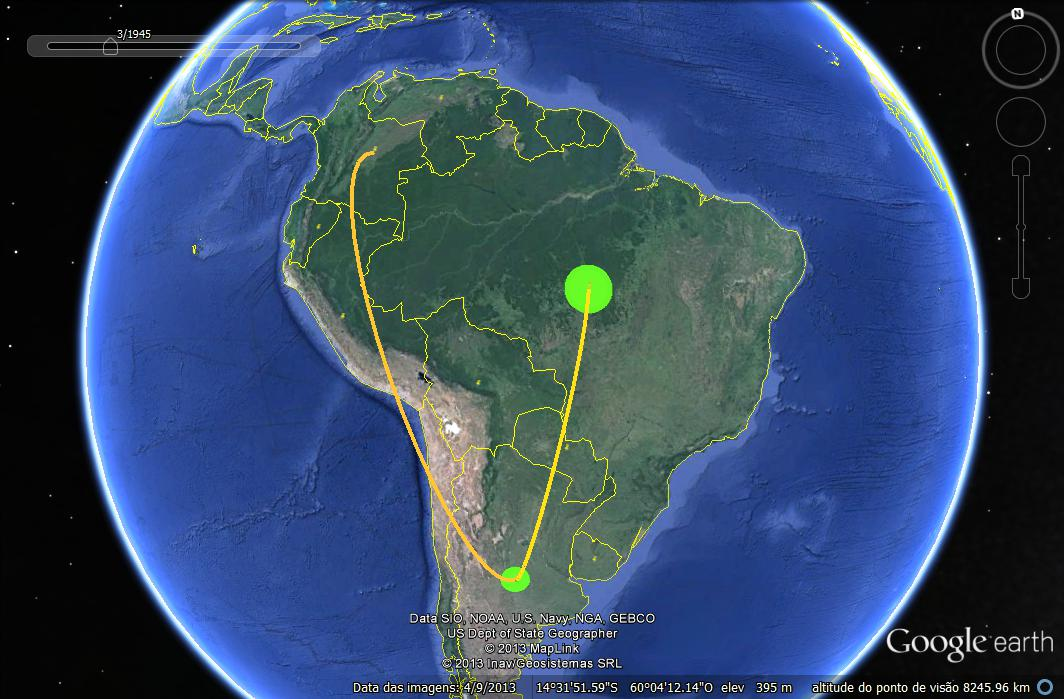
\includegraphics[scale=.20]{FIGURES/A_1945.jpg}}
\subfigure[O -- $1995$ ]{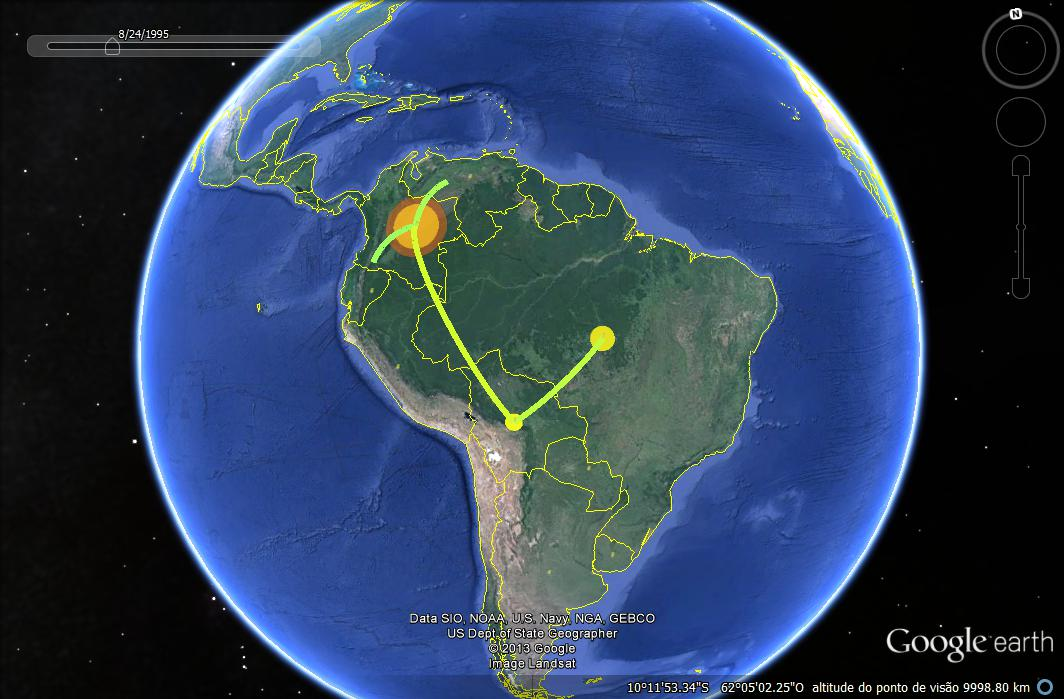
\includegraphics[scale=.20]{FIGURES/O_1995.jpg}}\\
\subfigure[A -- $1965$ ]{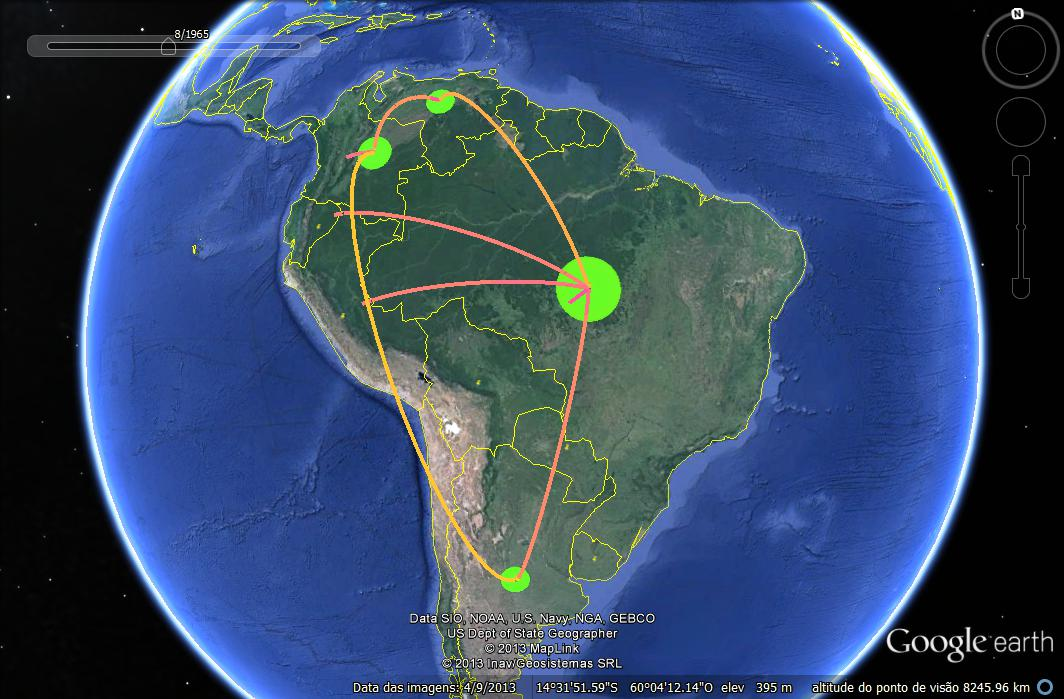
\includegraphics[scale=.20]{FIGURES/A_1965.jpg}}
\subfigure[O -- $2000$ ]{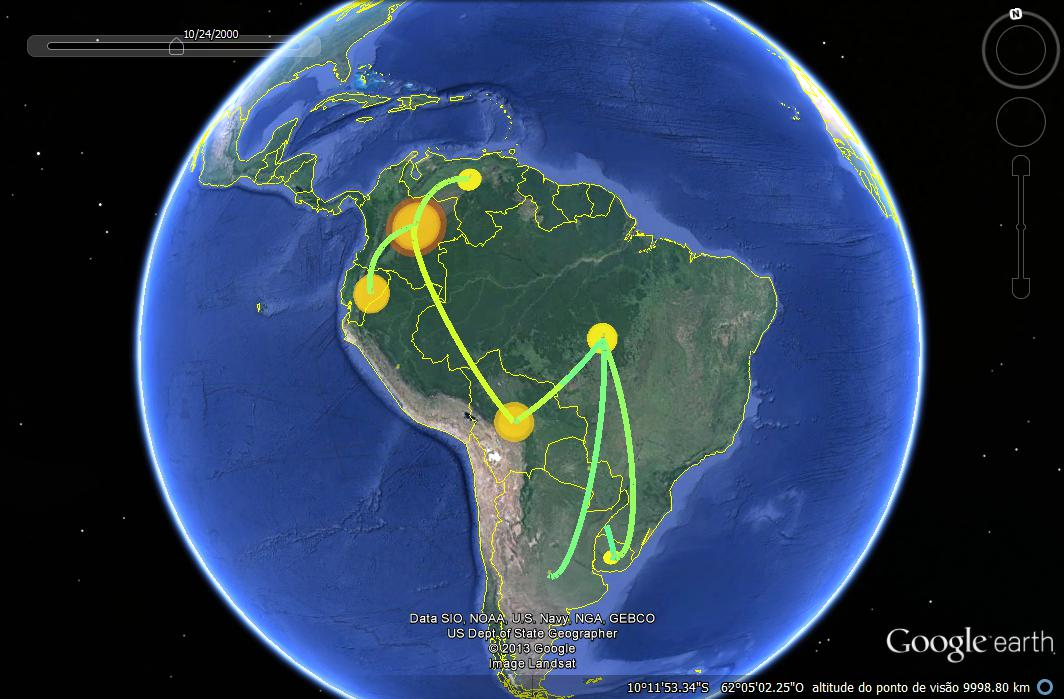
\includegraphics[scale=.20]{FIGURES/O_2000.jpg}}\\
\subfigure[A -- $1980$ ]{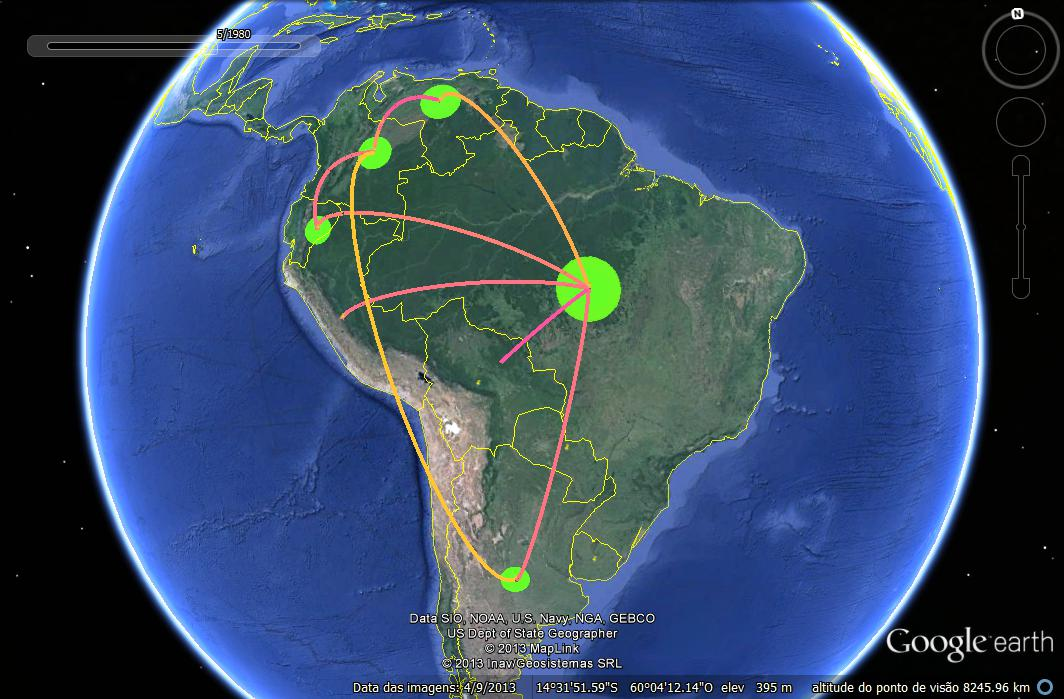
\includegraphics[scale=.20]{FIGURES/A_1980.jpg}}
\subfigure[O -- $2005$ ]{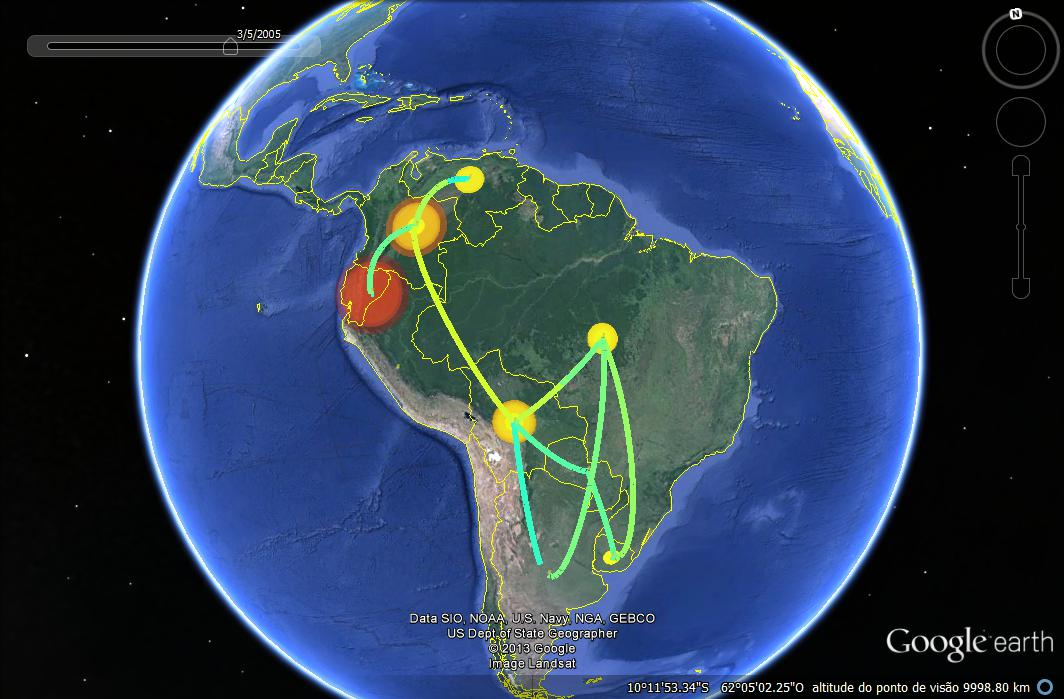
\includegraphics[scale=.20]{FIGURES/O_2005.jpg}}\\
\subfigure[A -- $2008$ ]{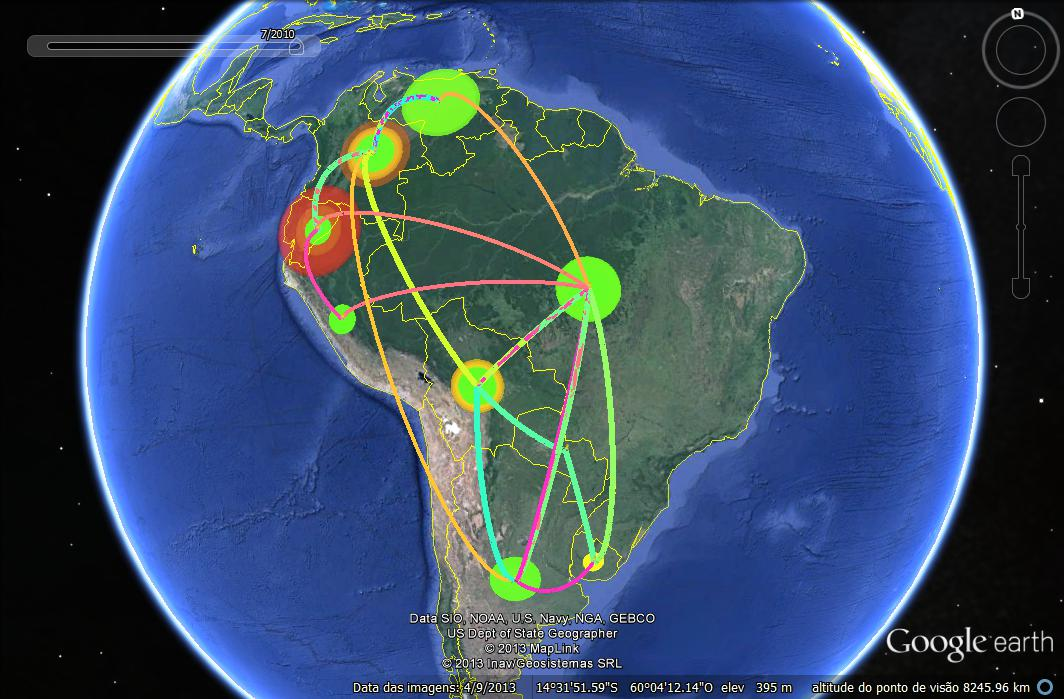
\includegraphics[scale=.20]{FIGURES/A_2008.jpg}}
\subfigure[O -- $2010$ ]{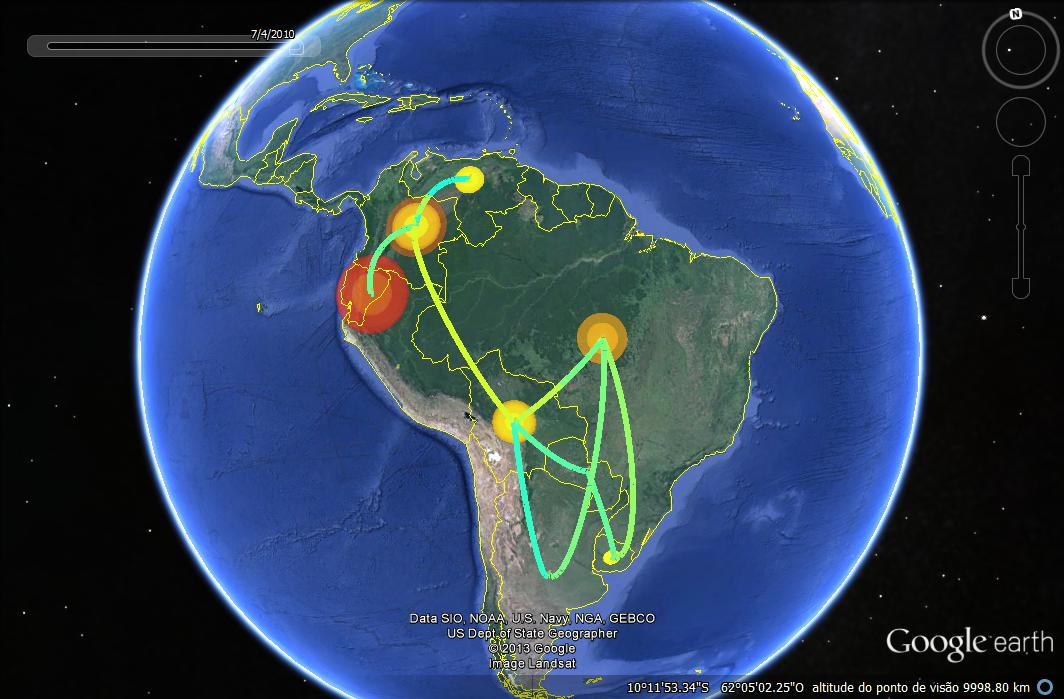
\includegraphics[scale=.20]{FIGURES/O_2010.jpg}}
\end{center}
\caption{}
\label{fig:migration}
\end{figure}
%%%%%%%%%%%%%%%%%%%%%%%%%%
%%%%%%%%%%%%%%%%%%%%%%%%%%
\newpage
\begin{figure}[H]
\begin{center}
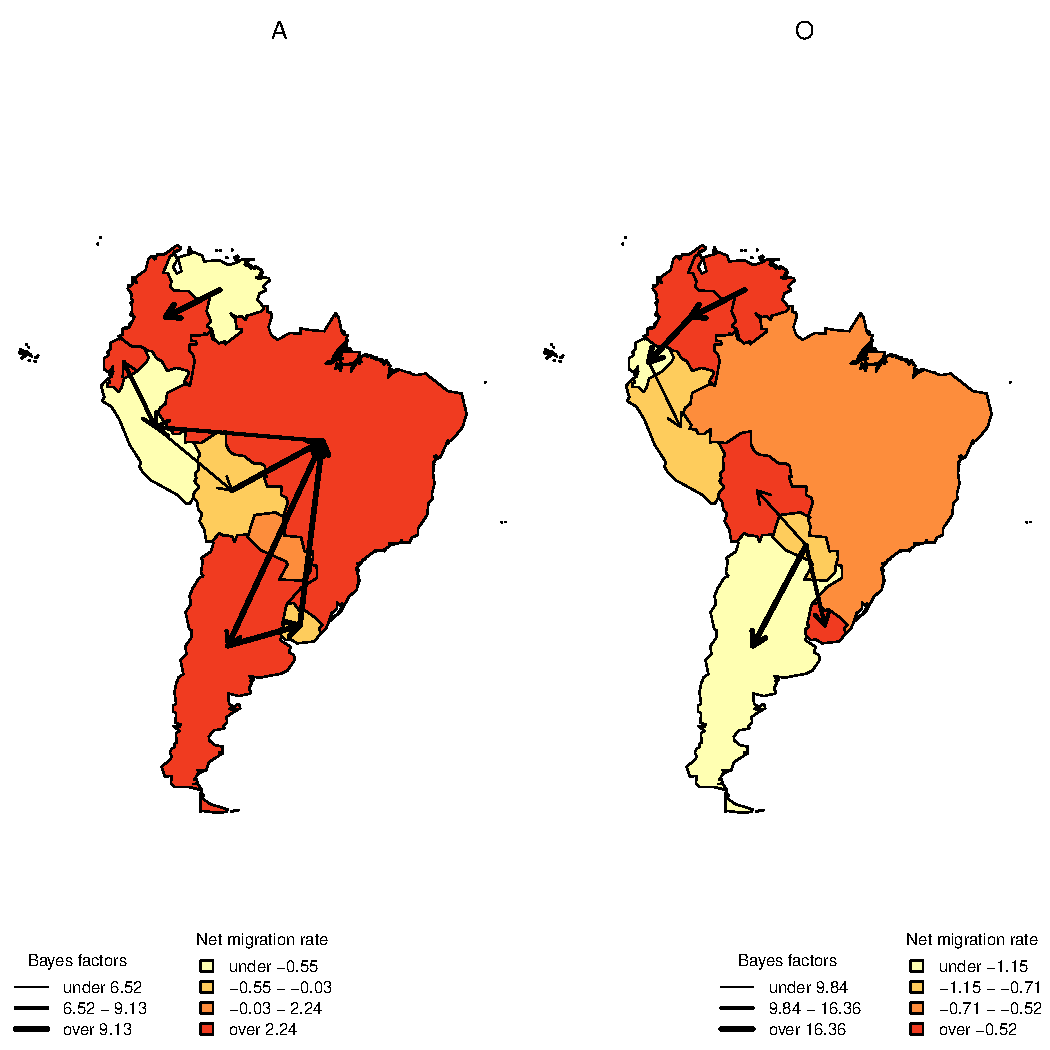
\includegraphics[scale=.90]{FIGURES/MJandBFs.pdf}
\end{center}
\caption{}
\label{fig:mj&BFs}
\end{figure}
%%%%%%%%%%%%%%%%%%%%%%%%%%
%%%%%%%%%%%%%%%%%%%%%%%%%%
\newpage
\begin{figure}[H]
\begin{center}
\subfigure[][]{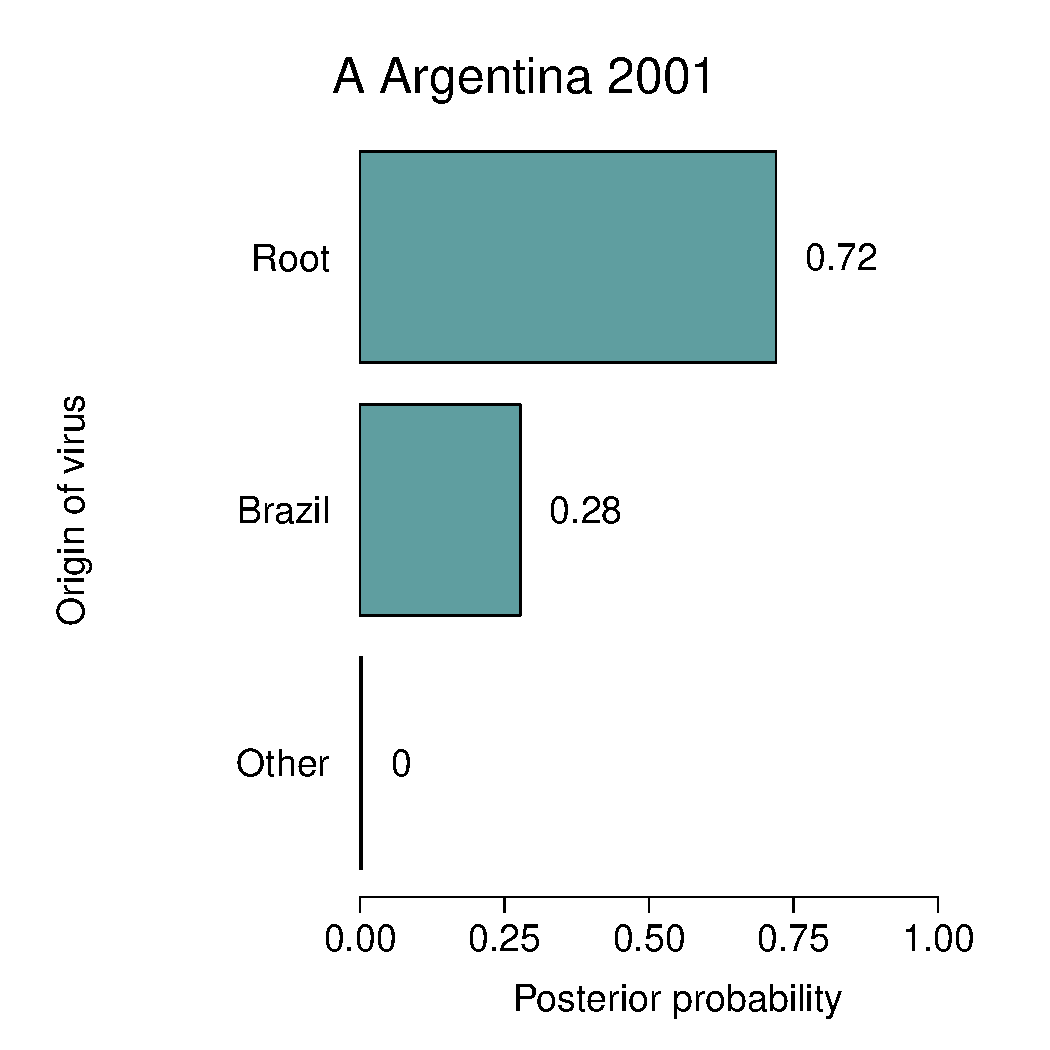
\includegraphics[scale=.40]{FIGURES/Origins_A_Argentina_2001.pdf}}
\subfigure[][]{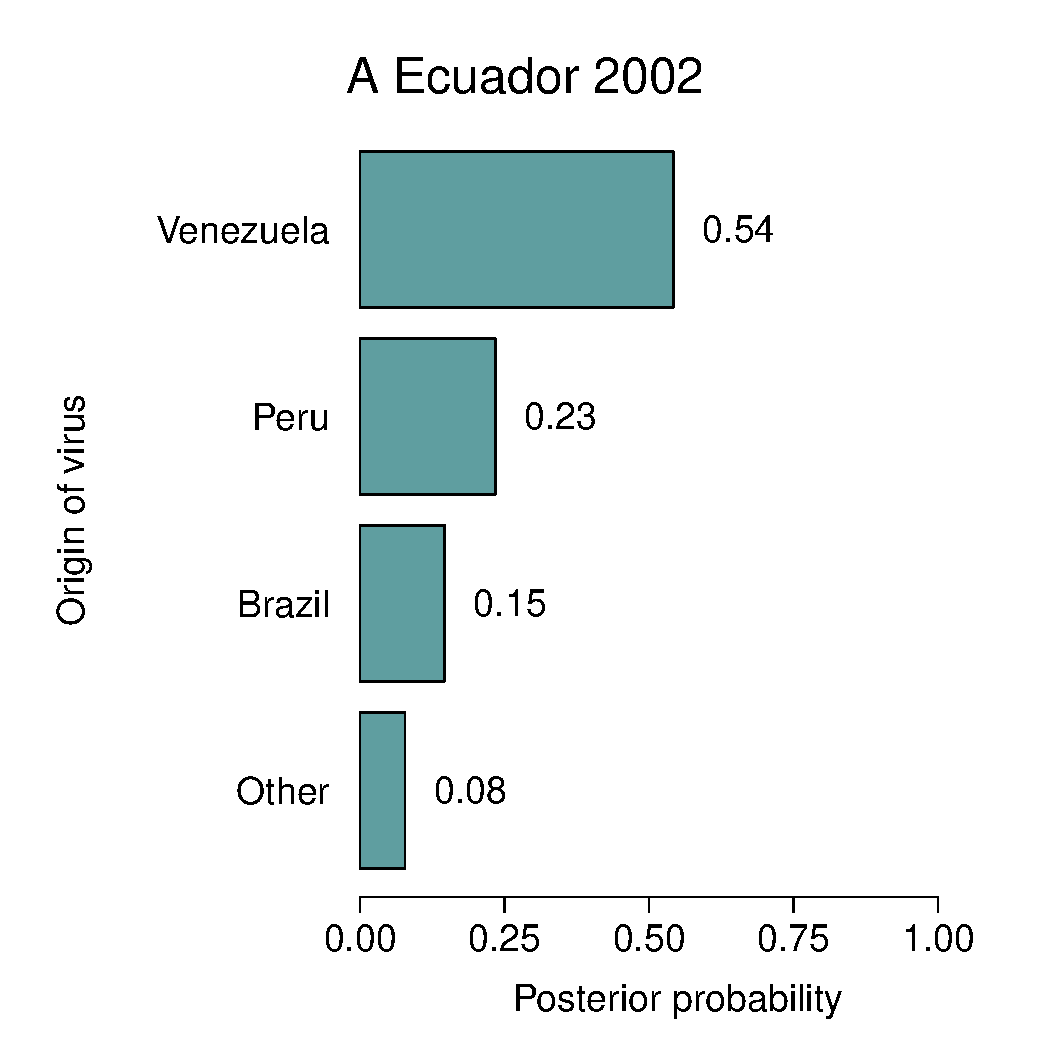
\includegraphics[scale=.40]{FIGURES/Origins_A_Ecuador_2002.pdf}}\\
\subfigure[][]{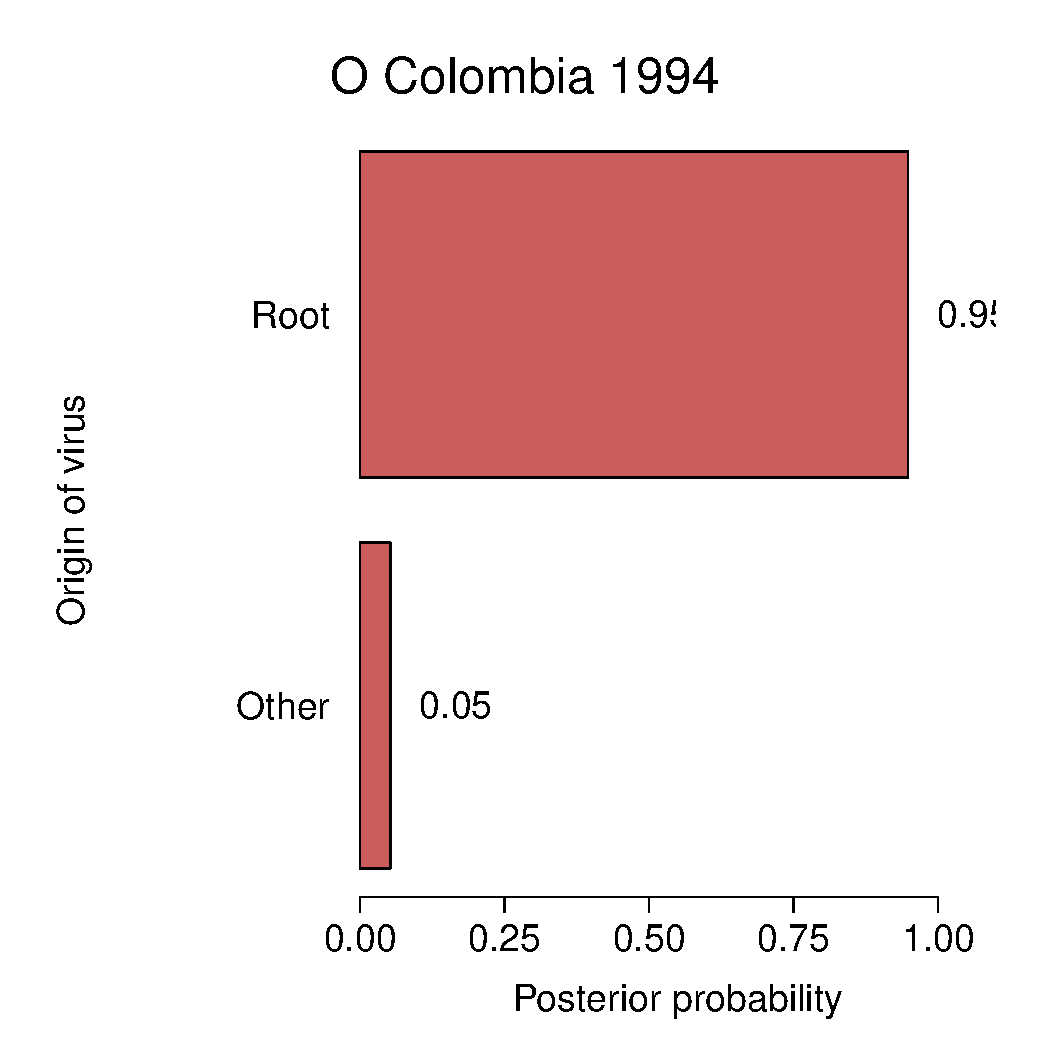
\includegraphics[scale=.40]{FIGURES/Origins_O_Colombia_1994.pdf}}
\subfigure[][]{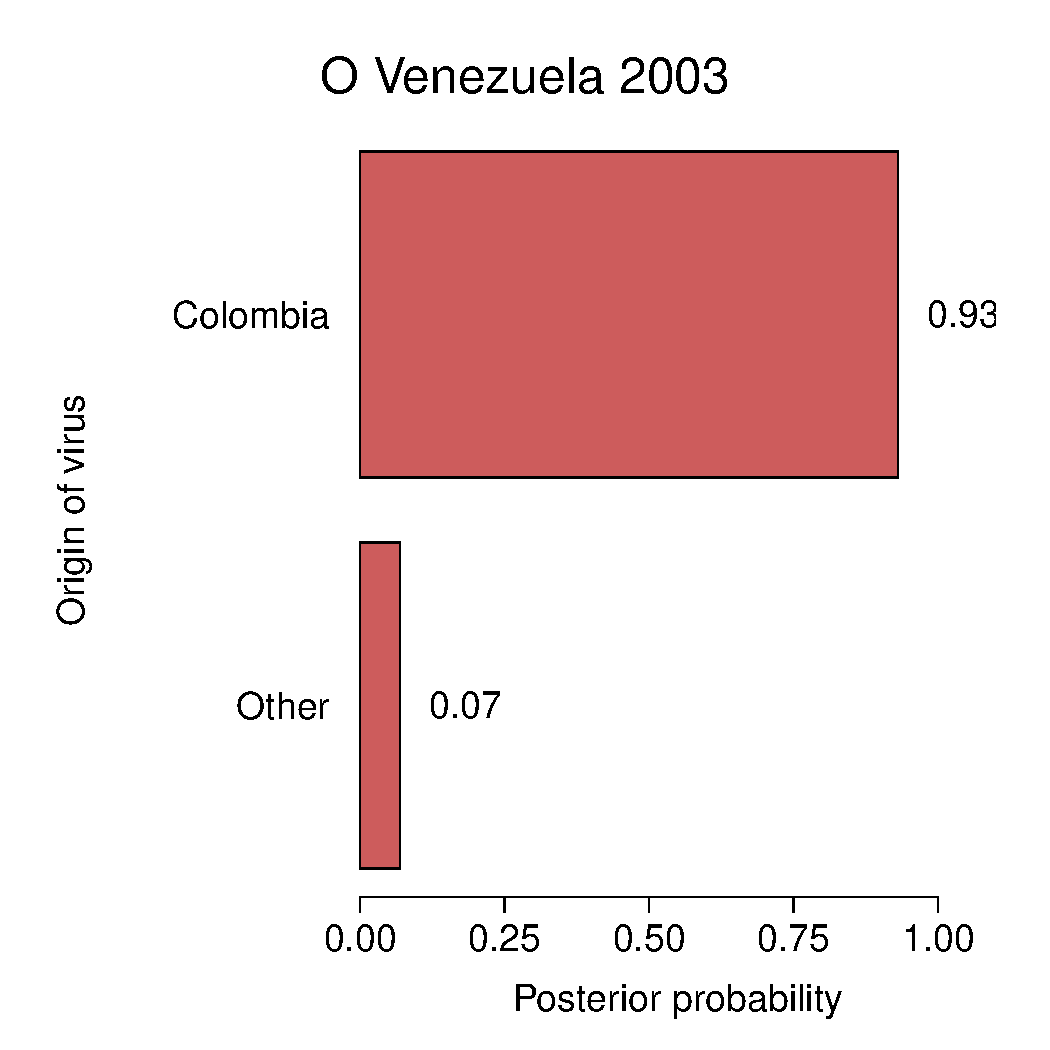
\includegraphics[scale=.40]{FIGURES/Origins_O_Venezuela_2003.pdf}}
\end{center}
\caption{}
\label{fig:epidemictracing}
\end{figure}
%%%%%%%%%%%%%%%%%%%%%%%%%%
%%%%%%%%%%%%%%%%%%%%%%%%%%
\newpage
\begin{figure}[H]
\begin{center}
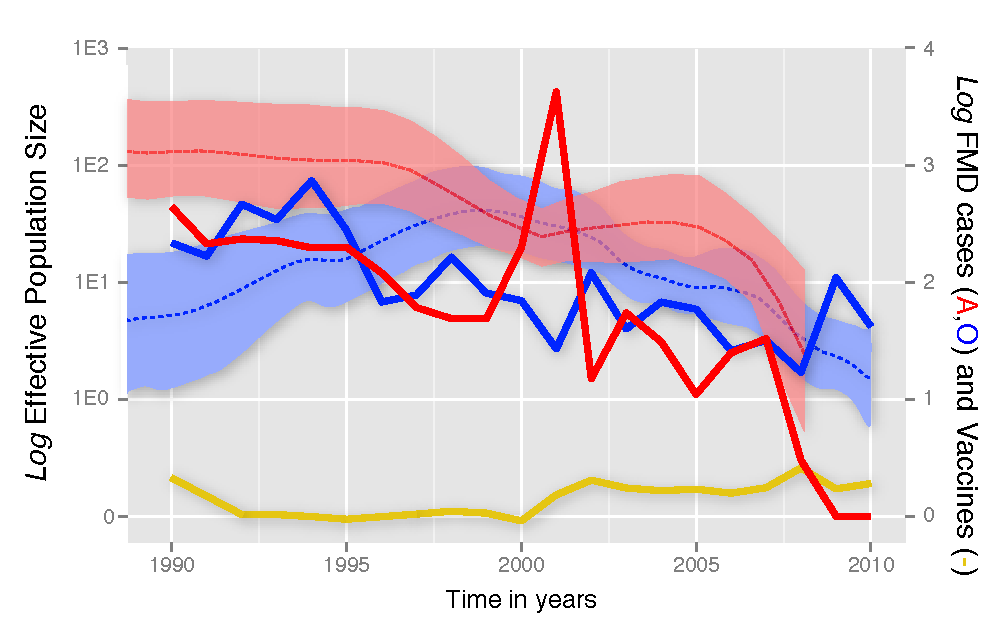
\includegraphics[scale=1.0]{FIGURES/skyride.pdf}
\end{center}
\caption{}
\label{fig:skyride}
\end{figure}
%%%%%%%%%%%%%%%%%%%%%%%%%%
%%%%%%%%%%%%%%%%%%%%%%%%%% 
\newpage
\begin{table}[H]
\caption{
\textbf{Spatial model selection results for epidemiological predictors.}
We assessed the significance of livestock trade in FMDV spread in South America using two marginal likelihood calculation methods, path sampling (PS) and stepping-stone sampling (SS), to estimate (log) marginal likelihoods for each predictor using $64$ path steps and $2$ million iterations per path step, and corresponding Bayes factor (BF) comparisons.
We also present the (log) marginal likelihood estimates for two location priors under which the location rates are estimated, rather than being fixed (as for the livestock predictors).
These results show that inverse-geographic distance is a strong predictor of viral spread for both serotypes.
Interestingly, while the best predictor for serotype O was the trade of cattle, this predictor failed to yield outperform the equal-rates prior.
These results provide evidence that the spread determinants of serotypes A and O are different in the continent.
}
\begin{center}
\begin{tabular}{lrrrrrr}
\toprule
 & \multicolumn{3}{c}{Serotype A}& \multicolumn{3}{c}{Serotype O}\\
 \midrule
Predictor & PS & SS & log BF$^2$ & PS & SS & log BF \\
%\hline
Cattle&-12588.76&-12591.26&-27.70&\textbf{-8308.94}&\textbf{-8311.21}& \textbf{13.49}\\
Distance&\textbf{-12557.69}&\textbf{-12559.73}&\textbf{3.83}&-8313.89&-8315.37&9.33\\
Pigs&-12589.33&-12590.94&-27.38&-8325.39&-8326.63&-1.93\\
Sheep&-12570.67&-12572.56&-9.00&-8326.23&-8330.64&-5.94\\
\\
\hline
Equal rates &-12561.98&-12563.56&--&-8321.49&-8324.70&--\\
\bottomrule
\end{tabular}
\end{center}
\begin{flushleft}
\end{flushleft}
\label{tab:preds}
 \end{table}
%%%%%%%%%%%%%%%%%%%%%%%%
%%%%%%%%%%%%%%%%%%%%%%%%
\newpage
\begin{table}[H]
\caption{
\textbf{Inferred root locations for each predictor for both serotypes.} We present most probable country of origin inferred using each predictor, with associated probabilities inside parentheses. 1-- all rates equal; 2-- Probability of being the root; 3-- Kullback-Leibler Divergence.
It can be noticed that there is considerable disagreement between predictors as to which is the most probable root of the circulating strains for serotype A.
The results for serotype O in the other hand consistently point Colombia as the source of the isolates analyzed.
We use the Kullback-Liebler divergence of the posterior distribution at root to an uniform distribution as a measure of spatial signal extraction~\cite{roots}.
By this criterion, the trade of pigs and sheep  for serotypes A and O respectively, are the most efficient predictors at capturing spatial signal.
}
\begin{center}
\begin{tabular}{lcccc}
\toprule
& \multicolumn{2}{c}{Serotype A}&\multicolumn{2}{c}{Serotype O}\\
Predictor& Origin ($Pr$(root)$^2$)& KL$^3$&Origin ($Pr$(root))& KL\\
\midrule
Distance & Argentina ($0.75$)& $3.86$ & Colombia ($0.96$)& $3.76$\\
Sheep    & Brazil ($0.89$) & $3.52$ & Colombia ($0.99$)& $5.91$\\
Pigs      & Colombia ($0.99$)& $5.98$& Colombia ($0.91$)& $4.73$\\
Equal rates$^1$  & Argentina ($0.84$)& $3.78$ &Colombia  ($0.96$)& $3.20$\\
Cattle   & Peru ($0.93$)& $5.17$ & Colombia ($0.95$)& $3.81$\\
 \bottomrule
\end{tabular}
\end{center}
\begin{flushleft}
\end{flushleft}
\label{tab:roots}
 \end{table}
%%%%%%%%%%%%%%%%%%%%%%%%
\end{document}
